\documentclass[11pt,a4paper]{article}

% Packages 
\usepackage[a4paper, margin=1in]{geometry}
\usepackage{libertinus}
\usepackage[T1]{fontenc}
\usepackage{graphicx}
\usepackage{booktabs}
\usepackage{longtable}
\usepackage{array}
\usepackage{multirow}
\usepackage{xcolor}
\usepackage{listings}
\usepackage{caption}
\usepackage{subcaption}
\usepackage{hyperref}
\usepackage{titlesec}
\usepackage{fancyhdr}
\usepackage{setspace}
\usepackage{enumitem}
\usepackage{float}
\usepackage{tabularx}
\usepackage{colortbl}
\usepackage{amsmath}
\usepackage{tocloft}
\usepackage{parskip}
\usepackage[stretch=20,shrink=20]{microtype}
\usepackage{tikz}
\usetikzlibrary{shapes.geometric, arrows.meta, positioning, calc, fit, backgrounds}

% Disable hyphenation and enable character-spacing expansion for MS Word-like justification
\hyphenpenalty=10000
\exhyphenpenalty=10000
\emergencystretch=2em

% Colors 
\definecolor{headerblue}{RGB}{31, 73, 125}
\definecolor{lightblue}{RGB}{189, 215, 238}
\definecolor{darkgray}{RGB}{64, 64, 64}
\definecolor{codegreen}{RGB}{0, 128, 0}
\definecolor{codegray}{RGB}{128, 128, 128}
\definecolor{codeblue}{RGB}{0, 0, 200}
\definecolor{codered}{RGB}{180, 0, 0}
\definecolor{codebg}{RGB}{245, 245, 245}
\setstretch{.95}

\hypersetup{
    colorlinks=true,
    linkcolor=headerblue,
    urlcolor=headerblue,
    citecolor=headerblue,
    pdftitle={ScholarFlow - Final Project Report},
    pdfauthor={ScholarFlow Team}
}

% Code Listing Styling
\lstdefinestyle{codeStyle}{
    backgroundcolor=\color{codebg},
    commentstyle=\color{codegreen},
    keywordstyle=\color{codeblue}\bfseries,
    numberstyle=\tiny\color{codegray},
    stringstyle=\color{codered},
    basicstyle=\ttfamily\footnotesize,
    breakatwhitespace=false,
    breaklines=true,
    captionpos=b,
    keepspaces=true,
    numbers=left,
    numbersep=6pt,
    showspaces=false,
    showstringspaces=false,
    showtabs=false,
    tabsize=2,
    frame=single,
    rulecolor=\color{black!15}
}
\lstset{style=codeStyle}

\titleformat{\chapter}[block]
  {\normalfont\fontsize{18}{20}\selectfont\bfseries\color{headerblue}}
  {\thechapter.}{0.5em}{}
\titlespacing*{\chapter}{0pt}{-30pt}{5pt}

\titleformat{\section}
  {\normalfont\fontsize{16}{18}\selectfont\bfseries\color{headerblue}}
  {\thesection}{0.5em}{}
\titleformat{\subsection}
  {\normalfont\fontsize{14}{16}\selectfont\bfseries\color{darkgray}}
  {\thesubsection}{0.5em}{}
\titleformat{\subsubsection}
  {\normalfont\fontsize{12}{14}\selectfont\bfseries\color{darkgray}}
  {\thesubsubsection}{0.5em}{}

\captionsetup{font=normalsize}

\setlength{\parskip}{4pt}

\onehalfspacing
\begin{document}

\begin{titlepage}
\centering
\vspace*{0.5cm}
\centerline{\makebox[\textwidth][c]{\LARGE \textbf{MILITARY INSTITUTE OF SCIENCE AND TECHNOLOGY}}}
\vspace{.4cm}
\includegraphics[width=0.5\textwidth]{mistlogo.png}\\[0.4cm]
\resizebox{\linewidth}{!}{\textbf{DEPARTMENT OF COMPUTER SCIENCE AND ENGINEERING}}\\[0.6cm]

{\large \textbf{\textsc{CSE 464: Software Development Projet-II}}}\\[0.3cm]
{\small \textcolor{darkgray}{\textsc{Final Project Report}}}\\[0.2cm]
{\small \textcolor{darkgray}{of}}\\[0.3cm]
{\Huge \textbf{\textcolor{headerblue}{\textsc{SCHOLARFLOW}}}}\\[0.2cm]
{\small \textit{\textcolor{darkgray}{\textsc{An AI-Assisted Academic Literature Review and Collaborative Research Workspace}}}}\\[0.3cm]

{\large \textbf{\textcolor{headerblue}{\textsc{Group:}}} B5 \quad \textbf{\textcolor{headerblue}{\textsc{Section:}}} B}\\[0.8cm]
\begin{table}[h]
\centering
\small
\begin{tabular*}{\textwidth}{@{} l l @{\extracolsep{\fill}} l @{}}
\textbf{\textcolor{headerblue}{\textsc{Submitted By}}} & & \textbf{\textcolor{headerblue}{\textsc{Submitted To}}} \\ [1.5ex]
\textcolor{darkgray}{\textsc{Lt Sizdatul Karim Evan}} & \textcolor{darkgray}{202214163} & \textcolor{darkgray}{\textsc{Lt Col Md Abul Basar}} \\[0.6ex]
\textcolor{darkgray}{\textsc{Labiba Ibnat Matin}} & \textcolor{darkgray}{202314061} & \textcolor{darkgray}{\textsc{Prof. Dr. Md Mahbubur Rahman}} \\[0.6ex]
\textcolor{darkgray}{\textsc{Sabit Siraji}} & \textcolor{darkgray}{202314104} & \textcolor{darkgray}{\textsc{Asso. Prof. Dr. T M Shahriar Sazzad}} \\[0.6ex]
\textcolor{darkgray}{\textsc{Md Tamimul Islam}} & \textcolor{darkgray}{202314113} & \textcolor{darkgray}{\textsc{Lec Nafisa Maliyat}} \\[0.6ex]\\
\end{tabular*}
\end{table}

\vfill

{\large \textcolor{darkgray}{\textbf{Submission Date:} \today}}

\end{titlepage}

\pagenumbering{gobble}
\tableofcontents
\clearpage

\pagenumbering{arabic}
\setcounter{page}{1}
\pagestyle{plain}

% ==============================================================================
% 1. INTRODUCTION
% ==============================================================================
\section{Introduction}

\subsection{Project Title}
\textbf{ScholarFlow: An AI-Assisted Academic Literature Review and Collaborative Research Workspace}

\subsection{Brief Overview}
Conducting a comprehensive academic literature review is one of the most time-consuming steps of any research project. Researchers typically browse search engines to find relevant papers, read dozens of abstracts to filter out off-topic work, build comparison tables manually, find open research gaps, and organize their draft sections using fragmented tools. When working in teams, sharing working drafts over generic cloud documents frequently leads to accidental overwrites and confusion over who owns which section.

ScholarFlow was developed to address these exact problems in a single unified system. It combines an academic search pipeline, an automated multi-agent research workflow, and a structured multi-user workspace. Users can enter a research question or topic into the application. The system then automatically plans academic search queries, fetches real peer-reviewed papers from the Semantic Scholar database, summarizes key contributions, constructs side-by-side methodology comparisons, extracts open research gaps, and drafts a structured narrative literature review.

In addition to automated generation, ScholarFlow functions as a multi-user collaborative workspace. Research teams can divide responsibilities across four primary draft sections (Abstract, Introduction, Literature Review, and Methodology). Team members who do not own a given section can draft proposals using an in-app split-view editor and submit formal edit requests. Assigned section owners review and merge these proposals directly into the approved draft, while project owners maintain complete version snapshots for milestones and rollbacks.

\subsection{Target Users}
ScholarFlow is designed specifically for:
\begin{itemize}
    \item \textbf{Undergraduate and Postgraduate Students:} Students working on thesis proposals, capstone projects, or term research papers who need a structured workflow to discover relevant literature, compare methodologies, and draft their related works section.
    \item \textbf{Academic Research Teams and Lab Groups:} Faculty, graduate research assistants, and co-authors who must divide section-writing duties and peer-review each other's contributions without write collisions.
    \item \textbf{Independent Scholars and Industry R\&D Teams:} Professionals surveying technical domains who need quick, citation-grounded summaries, comparative tables, and identification of unsolved problems without reading hundreds of PDF files manually.
\end{itemize}

% ==============================================================================
% 2. USER REQUIREMENTS AND DEVELOPED FEATURES
% ==============================================================================
\section{User Requirements and Developed Features}

\subsection{User Roles}
The application supports four distinct user roles, enforced by backend permission validation:
\begin{enumerate}
    \item \textbf{Project Owner (Leader):} The user who creates the research project. The project owner holds administrative authority over the workspace: assigning section owners, inviting collaborators by email, updating project timelines, approving or rejecting section changes, and saving or rolling back project version snapshots.
    \item \textbf{Section Owner (Assigned Co-Author):} A project collaborator assigned by the project owner to be responsible for a specific paper section (Abstract, Introduction, Literature Review, or Methodology). Section owners can edit their section's approved content directly and have exclusive authority to approve or reject edit requests submitted by other team members for that section.
    \item \textbf{Collaborator / Contributor (Editor):} A verified project member who is not the assigned owner of a given section. They can view the section, draft changes in a private working draft copy, and submit formal edit requests to the section owner for review.
\end{enumerate}

\subsection{Requirements and Implemented Features Mapping}
Table~\ref{tab:requirements} maps the key user requirements and roles to the developed features.

\begin{longtable}{p{4.5cm} p{3.2cm} p{7.5cm}}
\caption{User Requirements and Implemented System Features} \label{tab:requirements} \\
\toprule
\textbf{User Requirement} & \textbf{User Role} & \textbf{Implemented Feature} \\
\midrule
\endfirsthead
\toprule
\textbf{User Requirement} & \textbf{User Role} & \textbf{Implemented Feature} \\
\midrule
\endhead
\bottomrule
\endfoot

Secure account registration and profile management & All Users & Supabase Auth integration with email/password authentication, user profile management, avatar support, university affiliation, and aggregated citation analytics. \\
\addlinespace
Automated academic paper retrieval from natural language queries & All Roles & Query Planning Agent produces academic query variations; Search Agent queries the Semantic Scholar Graph API, fetching titles, authors, DOIs, abstracts, publication years, and citation counts. \\
\addlinespace
Interactive paper repository and manual curation & All Roles & Repository view allowing users to toggle paper selection flags, inspect full abstracts, view DOIs, and filter which papers feed into the synthesis agents. \\
\addlinespace
Automated structured summarization and comparison & All Roles & Summary and Comparison Agents process selected abstracts to generate unified key takeaways, methodology comparisons, and metric evaluations. \\
\addlinespace
Automated research gap extraction and literature review drafting & All Roles & Research Gap and Literature Review Agents detect open problems and synthesize a complete multi-paragraph narrative review grounded in retrieved papers. \\
\addlinespace
Flexible execution of individual workflow steps & All Roles & Router Agent and LangGraph workflow allowing users to execute either the full pipeline or jump directly into specific sub-agents (e.g., summary only). \\
\addlinespace
Team collaboration and member invitation & Project Owner & In-app email invitation system using secure random tokens. Collaborators view incoming invitations in their personal inbox and accept or decline. \\
\addlinespace
Collaborative section drafting without write collisions & Section Owners and Collaborators & Four dedicated project sections (Abstract, Introduction, Literature Review, Methodology). Section owners edit directly; other members submit edits via an approval queue. \\
\addlinespace
Working draft management and version history & Section Owners and Collaborators & Section Versioning and Split-View Editor allowing collaborators to save timestamped local working versions before submitting for formal approval. \\
\addlinespace
Milestone snapshots and state restoration & Project Owner & Project-wide version snapshot system that captures all current outputs, selected papers, and section text into immutable snapshots with rollback capabilities. \\
\bottomrule
\end{longtable}

\clearpage

% ==============================================================================
% 3. ER DIAGRAM
% ==============================================================================
\section{Entity-Relationship (ER) Diagram}

The ScholarFlow database is built on PostgreSQL hosted via Supabase. Figure~\ref{fig:er_diagram} shows the complete relational schema, including all active tables, primary keys, foreign keys, and cardinalities.

\begin{figure}[H]
\centering
\noindent\resizebox{\linewidth}{!}{%
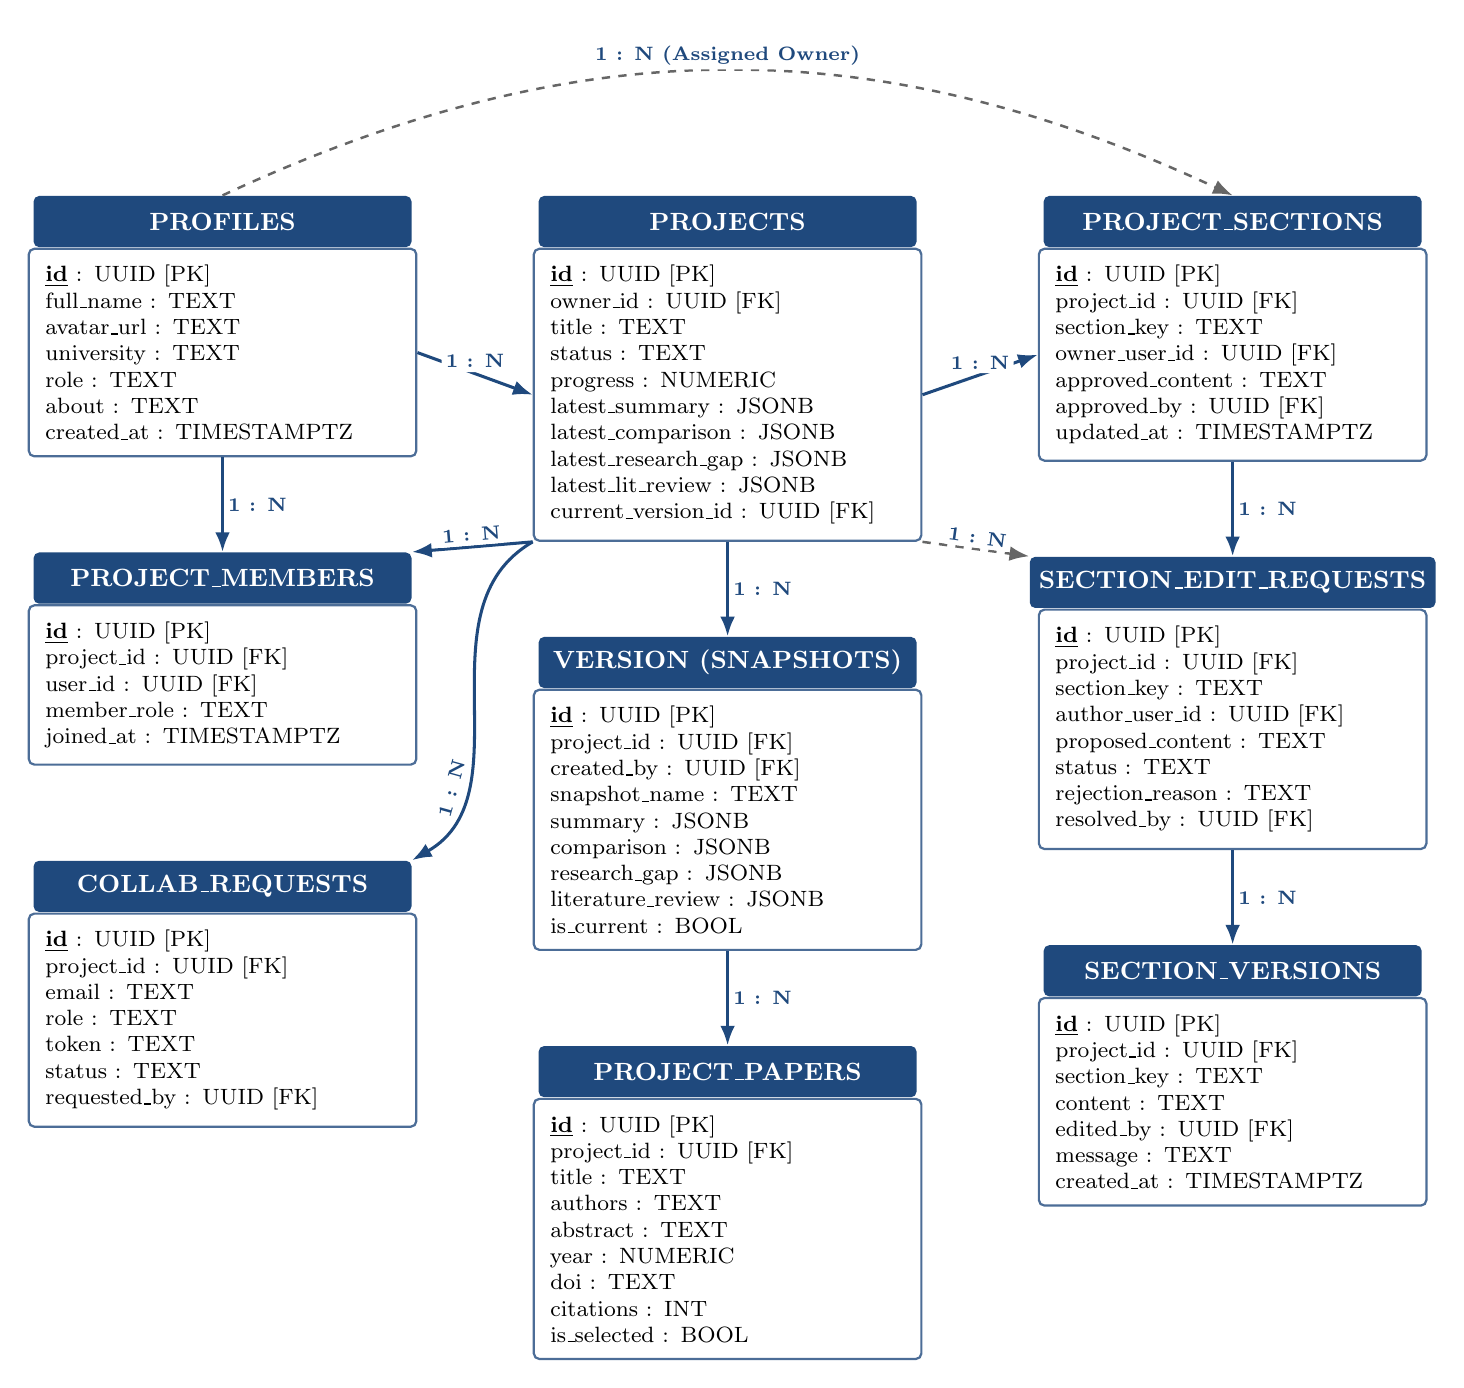
\begin{tikzpicture}[
    every node/.style={font=\small},
    tableheader/.style={
        rectangle, 
        fill=headerblue, 
        text=white, 
        font=\bfseries\small, 
        minimum width=4.8cm, 
        minimum height=0.65cm, 
        rounded corners=2pt, 
        text centered
    },
    tablebody/.style={
        rectangle, 
        draw=headerblue!80, 
        thick, 
        fill=white, 
        rounded corners=2pt, 
        inner sep=6pt, 
        text width=4.5cm,
        font=\footnotesize
    },
    rel/.style={
        -{Latex[length=2.5mm]}, 
        draw=headerblue, 
        thick,
        line width=1.1pt
    },
    relsub/.style={
        -{Latex[length=2.5mm]}, 
        draw=darkgray!80, 
        dashed,
        thick,
        line width=0.9pt
    },
    card/.style={
        font=\scriptsize\bfseries, 
        text=headerblue, 
        fill=white, 
        inner sep=1.5pt, 
        rounded corners=1pt
    }
]

% ==================== COLUMN 1: USERS & COLLABORATION ====================

% PROFILES
\node[tableheader] (profiles_hdr) at (0, 0) {\textsc{PROFILES}};
\node[tablebody, below=0cm of profiles_hdr] (profiles_body) {
    \textbf{\underline{id}} : UUID [PK] \\
    full\_name : TEXT \\
    avatar\_url : TEXT \\
    university : TEXT \\
    role : TEXT \\
    about : TEXT \\
    created\_at : TIMESTAMPTZ
};

% PROJECT_MEMBERS
\node[tableheader, below=1.2cm of profiles_body] (members_hdr) {\textsc{PROJECT\_MEMBERS}};
\node[tablebody, below=0cm of members_hdr] (members_body) {
    \textbf{\underline{id}} : UUID [PK] \\
    project\_id : UUID [FK] \\
    user\_id : UUID [FK] \\
    member\_role : TEXT \\
    joined\_at : TIMESTAMPTZ
};

% COLLABORATION_REQUESTS (INVITATIONS)
\node[tableheader, below=1.2cm of members_body] (collab_hdr) {\textsc{COLLAB\_REQUESTS}};
\node[tablebody, below=0cm of collab_hdr] (collab_body) {
    \textbf{\underline{id}} : UUID [PK] \\
    project\_id : UUID [FK] \\
    email : TEXT \\
    role : TEXT \\
    token : TEXT \\
    status : TEXT \\
    requested\_by : UUID [FK]
};


% ==================== COLUMN 2: CORE PROJECTS & PAPERS ====================

% PROJECTS
\node[tableheader, right=1.6cm of profiles_hdr] (projects_hdr) {\textsc{PROJECTS}};
\node[tablebody, below=0cm of projects_hdr] (projects_body) {
    \textbf{\underline{id}} : UUID [PK] \\
    owner\_id : UUID [FK] \\
    title : TEXT \\
    status : TEXT \\
    progress : NUMERIC \\
    latest\_summary : JSONB \\
    latest\_comparison : JSONB \\
    latest\_research\_gap : JSONB \\
    latest\_lit\_review : JSONB \\
    current\_version\_id : UUID [FK]
};

% VERSION (SNAPSHOTS)
\node[tableheader, below=1.2cm of projects_body] (version_hdr) {\textsc{VERSION (SNAPSHOTS)}};
\node[tablebody, below=0cm of version_hdr] (version_body) {
    \textbf{\underline{id}} : UUID [PK] \\
    project\_id : UUID [FK] \\
    created\_by : UUID [FK] \\
    snapshot\_name : TEXT \\
    summary : JSONB \\
    comparison : JSONB \\
    research\_gap : JSONB \\
    literature\_review : JSONB \\
    is\_current : BOOL
};

% PROJECT_PAPERS
\node[tableheader, below=1.2cm of version_body] (papers_hdr) {\textsc{PROJECT\_PAPERS}};
\node[tablebody, below=0cm of papers_hdr] (papers_body) {
    \textbf{\underline{id}} : UUID [PK] \\
    project\_id : UUID [FK] \\
    title : TEXT \\
    authors : TEXT \\
    abstract : TEXT \\
    year : NUMERIC \\
    doi : TEXT \\
    citations : INT \\
    is\_selected : BOOL
};


% ==================== COLUMN 3: SECTION DRAFTING & REVIEW ====================

% PROJECT_SECTIONS
\node[tableheader, right=1.6cm of projects_hdr] (sections_hdr) {\textsc{PROJECT\_SECTIONS}};
\node[tablebody, below=0cm of sections_hdr] (sections_body) {
    \textbf{\underline{id}} : UUID [PK] \\
    project\_id : UUID [FK] \\
    section\_key : TEXT \\
    owner\_user\_id : UUID [FK] \\
    approved\_content : TEXT \\
    approved\_by : UUID [FK] \\
    updated\_at : TIMESTAMPTZ
};

% PROJECT_SECTION_EDIT_REQUESTS
\node[tableheader, below=1.2cm of sections_body] (edit_req_hdr) {\textsc{SECTION\_EDIT\_REQUESTS}};
\node[tablebody, below=0cm of edit_req_hdr] (edit_req_body) {
    \textbf{\underline{id}} : UUID [PK] \\
    project\_id : UUID [FK] \\
    section\_key : TEXT \\
    author\_user\_id : UUID [FK] \\
    proposed\_content : TEXT \\
    status : TEXT \\
    rejection\_reason : TEXT \\
    resolved\_by : UUID [FK]
};

% SECTION_VERSIONS (LOCAL DRAFTS)
\node[tableheader, below=1.2cm of edit_req_body] (sec_ver_hdr) {\textsc{SECTION\_VERSIONS}};
\node[tablebody, below=0cm of sec_ver_hdr] (sec_ver_body) {
    \textbf{\underline{id}} : UUID [PK] \\
    project\_id : UUID [FK] \\
    section\_key : TEXT \\
    content : TEXT \\
    edited\_by : UUID [FK] \\
    message : TEXT \\
    created\_at : TIMESTAMPTZ
};


% ==================== RELATIONSHIPS & CONNECTORS ====================

% Profiles -> Projects (1:N Ownership)
\draw[rel] (profiles_body.east) -- node[card, above]{1 : N} (projects_body.west);

% Profiles -> Members (1:N)
\draw[rel] (profiles_body.south) -- node[card, right]{1 : N} (members_hdr.north);

% Projects -> Members (1:N)
\draw[rel] (projects_body.south west) -- node[card, above, sloped]{1 : N} (members_hdr.north east);

% Projects -> Collab Requests (1:N)
\draw[rel] (projects_body.south west) to[out=210, in=30] node[card, near end, above, sloped]{1 : N} (collab_hdr.north east);

% Projects -> Version (1:N)
\draw[rel] (projects_body.south) -- node[card, right]{1 : N} (version_hdr.north);

% Projects -> Project Papers (1:N)
\draw[rel] (version_body.south) -- node[card, right]{1 : N} (papers_hdr.north);

% Projects -> Sections (1:N)
\draw[rel] (projects_body.east) -- node[card, above]{1 : N} (sections_body.west);

% Sections -> Edit Requests (1:N)
\draw[rel] (sections_body.south) -- node[card, right]{1 : N} (edit_req_hdr.north);

% Sections -> Section Versions (1:N)
\draw[rel] (edit_req_body.south) -- node[card, right]{1 : N} (sec_ver_hdr.north);

% Projects -> Edit Requests (1:N)
\draw[relsub] (projects_body.south east) -- node[card, above, sloped]{1 : N} (edit_req_hdr.north west);

% Profiles -> Sections (owner_user_id FK)
\draw[relsub] (profiles_hdr.north) to[out=25, in=155] node[card, above]{1 : N (Assigned Owner)} (sections_hdr.north);

\end{tikzpicture}%
}
\caption{ScholarFlow Entity-Relationship (ER) Diagram displaying tables, primary keys, foreign keys, and cardinalities.}
\label{fig:er_diagram}
\end{figure}

\subsection{Database Entities Description}
\begin{itemize}
    \item \textbf{\texttt{profiles}:} Extends the Supabase \texttt{auth.users} table. Stores each user's full name, profile picture link, affiliated university, primary research role, and personal summary.
    \item \textbf{\texttt{projects}:} The core workspace record storing title, research description, timeline, current milestone status, cached JSON outputs from agents, and current active snapshot reference.
    \item \textbf{\texttt{project\_members}:} Connects users to projects with designated roles (\texttt{viewer}, \texttt{editor}, \texttt{lead}) to regulate permissions.
    \item \textbf{\texttt{collaboration\_requests}:} Manages email invitations sent to prospective collaborators, secured with unique random invitation tokens and status flags (\texttt{pending}, \texttt{accepted}, \texttt{declined}).
    \item \textbf{\texttt{project\_papers}:} Stores papers fetched from the Semantic Scholar API. Includes DOIs, citation counts, abstracts, publication years, and selection flags.
    \item \textbf{\texttt{version}:} Immutable snapshots of full project state, storing serialized AI outputs and paper collections for rollback capability.
    \item \textbf{\texttt{project\_sections}:} Tracks the current live approved text for the four main drafting sections (\texttt{abstract}, \texttt{introduction}, \texttt{literature\_review}, \texttt{methodology}) along with the assigned section owner.
    \item \textbf{\texttt{project\_section\_edit\_requests}:} Holds proposals submitted by non-owning team members awaiting approval or rejection from the section owner.
    \item \textbf{\texttt{section\_versions}:} Stores working draft versions saved by team members in the split-view editor before they request approval.
\end{itemize}

\clearpage
% ==============================================================================
% 4. ACTIVITY DIAGRAMS
% ==============================================================================
\section{Activity Diagrams}

This section details the primary interactions and decision workflows across three core system processes.

\subsection{Feature 1: Automated Multi-Agent Literature Review Pipeline}
Figure~\ref{fig:activity_agents} demonstrates how user inputs travel through the multi-agent backend pipeline from query generation to literature review synthesis.

\begin{figure}[H]
\centering
\noindent\resizebox{\linewidth}{!}{%
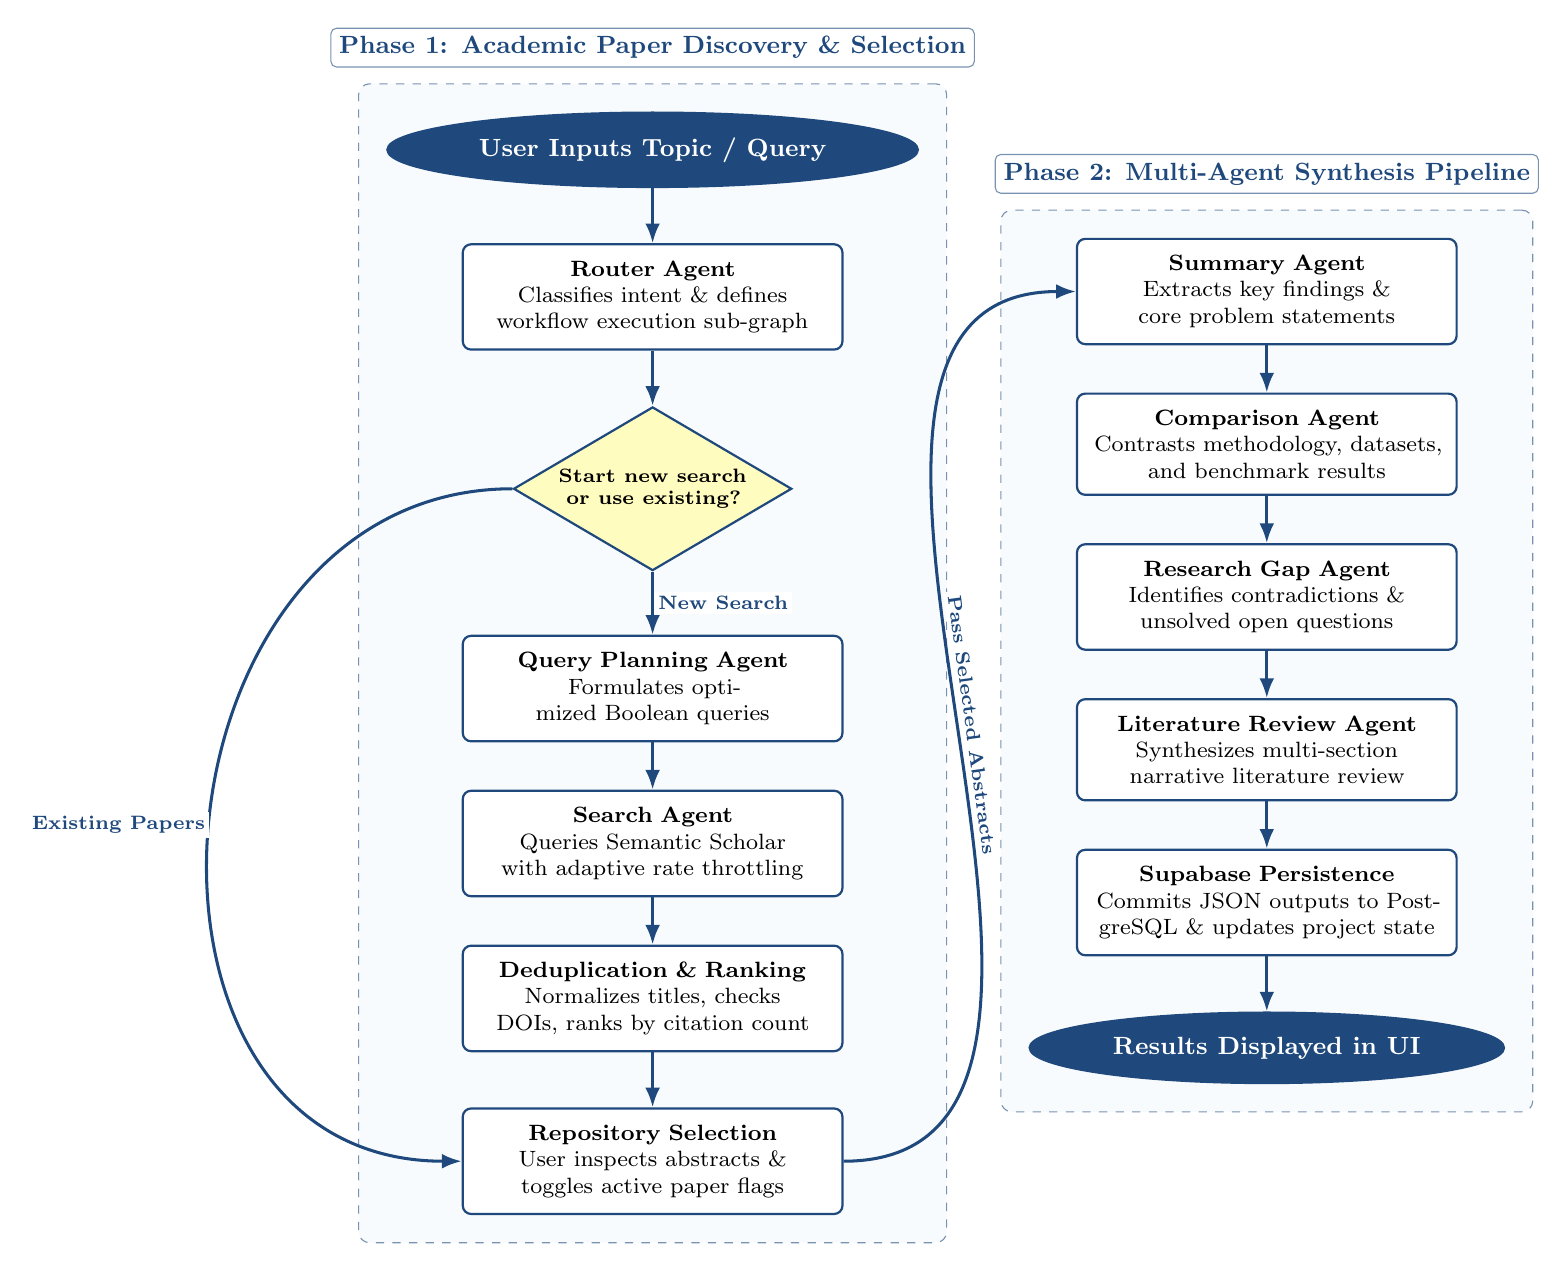
\begin{tikzpicture}[
    every node/.style={font=\small},
    phasebox/.style={
        rectangle, 
        draw=headerblue!60, 
        dashed, 
        fill=lightblue!10, 
        rounded corners=4pt, 
        inner sep=10pt
    },
    phasetitle/.style={
        font=\bfseries\small\color{headerblue}, 
        fill=white, 
        draw=headerblue!60, 
        rounded corners=2pt, 
        inner sep=3pt
    },
    startstop/.style={
        ellipse, 
        draw=headerblue, 
        thick, 
        fill=headerblue, 
        text=white, 
        font=\bfseries\small, 
        inner sep=5pt, 
        text centered
    },
    process/.style={
        rectangle, 
        draw=headerblue, 
        thick, 
        fill=white, 
        rounded corners=3pt, 
        text width=4.4cm, 
        text centered, 
        inner sep=6pt, 
        font=\footnotesize
    },
    decision/.style={
        diamond, 
        draw=headerblue, 
        thick, 
        fill=yellow!25, 
        text width=2.4cm, 
        text centered, 
        inner sep=1.5pt, 
        aspect=1.7, 
        font=\scriptsize\bfseries
    },
    arrow/.style={
        thick, 
        line width=1.1pt, 
        -{Latex[length=2.5mm]}, 
        draw=headerblue
    },
    edgecard/.style={
        font=\scriptsize\bfseries, 
        text=headerblue, 
        fill=white, 
        inner sep=1.5pt
    }
]

% ==================== PHASE 1: DISCOVERY & RETRIEVAL (LEFT) ====================

\node (start) [startstop] at (0, 0) {User Inputs Topic / Query};
\node (route) [process, below=0.7cm of start] {\textbf{Router Agent} \\ Classifies intent \& defines workflow execution sub-graph};
\node (decide_start) [decision, below=0.7cm of route] {Start new search or use existing?};

\node (query_plan) [process, below=0.8cm of decide_start] {\textbf{Query Planning Agent} \\ Formulates optimized Boolean queries};
\node (search_api) [process, below=0.6cm of query_plan] {\textbf{Search Agent} \\ Queries Semantic Scholar with adaptive rate throttling};
\node (dedup) [process, below=0.6cm of search_api] {\textbf{Deduplication \& Ranking} \\ Normalizes titles, checks DOIs, ranks by citation count};

\node (select) [process, below=0.7cm of dedup] {\textbf{Repository Selection} \\ User inspects abstracts \& toggles active paper flags};

% Connections Phase 1
\draw [arrow] (start) -- (route);
\draw [arrow] (route) -- (decide_start);
\draw [arrow] (decide_start) -- node[edgecard, right]{New Search} (query_plan);
\draw [arrow] (query_plan) -- (search_api);
\draw [arrow] (search_api) -- (dedup);
\draw [arrow] (dedup) -- (select);
\draw [arrow] (decide_start.west) to[out=180, in=180, looseness=1.4] node[edgecard, left]{Existing Papers} (select.west);


% ==================== PHASE 2: MULTI-AGENT SYNTHESIS (RIGHT) ====================

\node (summary) [process] at (7.8, -1.8) {\textbf{Summary Agent} \\ Extracts key findings \& core problem statements};
\node (compare) [process, below=0.6cm of summary] {\textbf{Comparison Agent} \\ Contrasts methodology, datasets, and benchmark results};
\node (gap) [process, below=0.6cm of compare] {\textbf{Research Gap Agent} \\ Identifies contradictions \& unsolved open questions};
\node (lit_review) [process, below=0.6cm of gap] {\textbf{Literature Review Agent} \\ Synthesizes multi-section narrative literature review};
\node (save_db) [process, below=0.6cm of lit_review] {\textbf{Supabase Persistence} \\ Commits JSON outputs to PostgreSQL \& updates project state};
\node (stop) [startstop, below=0.7cm of save_db] {Results Displayed in UI};

% Inter-Phase Connection
\draw [arrow] (select.east) to[out=0, in=180] node[edgecard, above, sloped]{Pass Selected Abstracts} (summary.west);

% Connections Phase 2
\draw [arrow] (summary) -- (compare);
\draw [arrow] (compare) -- (gap);
\draw [arrow] (gap) -- (lit_review);
\draw [arrow] (lit_review) -- (save_db);
\draw [arrow] (save_db) -- (stop);

% Visual Phase Grouping Boxes
\begin{scope}[on background layer]
    \node (box_p1) [phasebox, fit=(start) (select)] {};
    \node (title_p1) [phasetitle, above=0.2cm of box_p1.north] {\textsc{Phase 1: Academic Paper Discovery \& Selection}};

    \node (box_p2) [phasebox, fit=(summary) (stop)] {};
    \node (title_p2) [phasetitle, above=0.2cm of box_p2.north] {\textsc{Phase 2: Multi-Agent Synthesis Pipeline}};
\end{scope}

\end{tikzpicture}%
}
\caption{Activity Diagram for the Multi-Agent Literature Discovery and Synthesis Pipeline.}
\label{fig:activity_agents}
\end{figure}

\clearpage
\subsection{Feature 2: Role-Based Section Co-Authoring and Edit Approval Workflow}
Figure~\ref{fig:activity_collab} illustrates how team members collaborate on paper sections without overwriting each other's work.

\begin{figure}[H]
\centering
\noindent\resizebox{0.92\linewidth}{!}{%
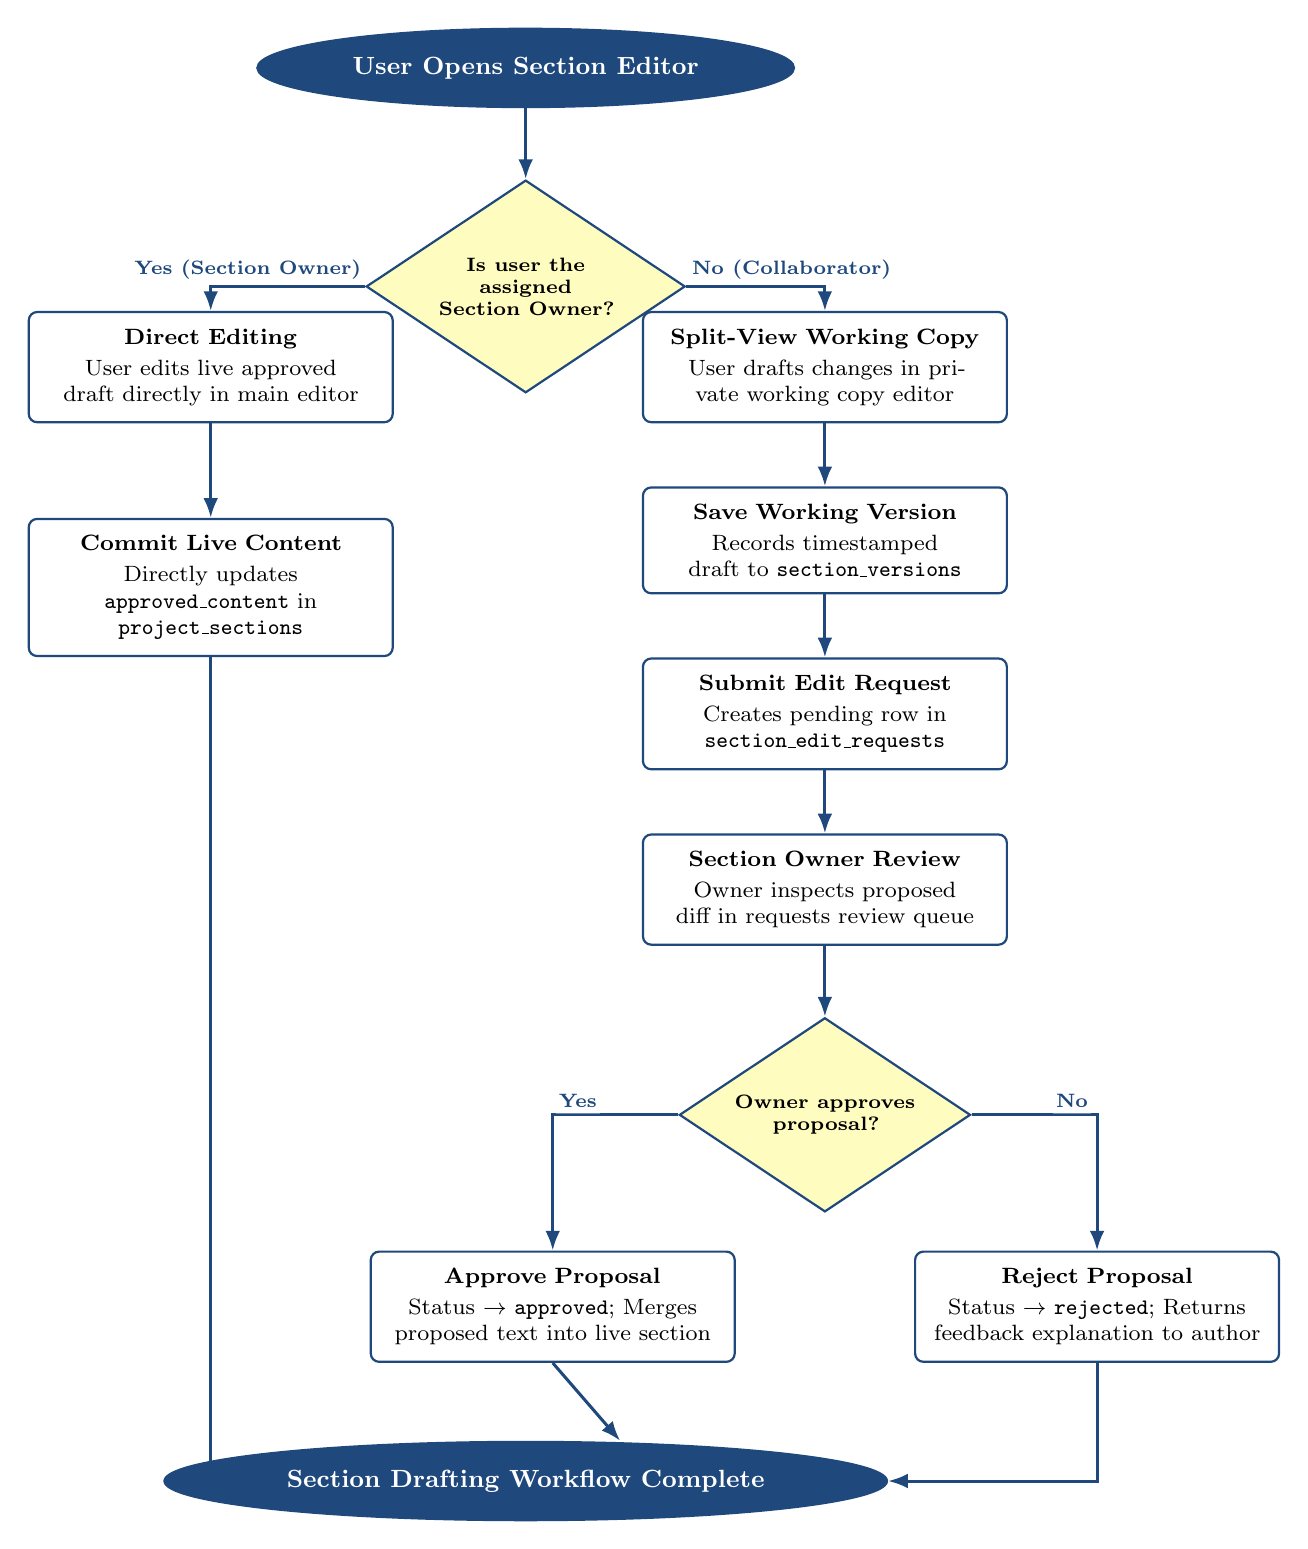
\begin{tikzpicture}[
    every node/.style={font=\small},
    startstop/.style={
        ellipse, 
        draw=headerblue, 
        thick, 
        fill=headerblue, 
        text=white, 
        font=\bfseries\small, 
        inner sep=6pt, 
        text centered
    },
    process/.style={
        rectangle, 
        draw=headerblue, 
        thick, 
        fill=white, 
        rounded corners=3pt, 
        text width=4.2cm, 
        text centered, 
        inner sep=6pt, 
        font=\footnotesize
    },
    decision/.style={
        diamond, 
        draw=headerblue, 
        thick, 
        fill=yellow!25, 
        text width=2.6cm, 
        text centered, 
        inner sep=2pt, 
        aspect=1.5, 
        font=\scriptsize\bfseries
    },
    arrow/.style={
        thick, 
        line width=1.1pt, 
        -{Latex[length=2.5mm]}, 
        draw=headerblue
    },
    edgecard/.style={
        font=\scriptsize\bfseries, 
        text=headerblue, 
        fill=white, 
        inner sep=2pt,
        rounded corners=1pt
    }
]

% ==================== TOP: START & INITIAL ROLE DECISION ====================
\node (start) [startstop] at (0, 0) {User Opens Section Editor};
\node (role_check) [decision, below=0.9cm of start] {Is user the assigned\\Section Owner?};

% ==================== LEFT BRANCH: SECTION OWNER PATH ====================
\node (direct_edit) [process] at (-4.0, -3.8) {
    \textbf{Direct Editing} \\[0.2em]
    User edits live approved draft directly in main editor
};
\node (direct_save) [process, below=1.2cm of direct_edit] {
    \textbf{Commit Live Content} \\[0.2em]
    Directly updates \texttt{approved\_content} in \texttt{project\_sections}
};

% ==================== RIGHT BRANCH: COLLABORATOR PATH ====================
\node (split_edit) [process] at (3.8, -3.8) {
    \textbf{Split-View Working Copy} \\[0.2em]
    User drafts changes in private working copy editor
};
\node (save_version) [process, below=0.8cm of split_edit] {
    \textbf{Save Working Version} \\[0.2em]
    Records timestamped draft to \texttt{section\_versions}
};
\node (submit_req) [process, below=0.8cm of save_version] {
    \textbf{Submit Edit Request} \\[0.2em]
    Creates pending row in \texttt{section\_edit\_requests}
};
\node (owner_review) [process, below=0.8cm of submit_req] {
    \textbf{Section Owner Review} \\[0.2em]
    Owner inspects proposed diff in requests review queue
};
\node (owner_decision) [decision, below=0.9cm of owner_review] {Owner approves\\proposal?};

\node (approve_action) [process, below left=1.1cm and 0.2cm of owner_decision] {
    \textbf{Approve Proposal} \\[0.2em]
    Status $\rightarrow$ \texttt{approved}; Merges proposed text into live section
};
\node (reject_action) [process, below right=1.1cm and 0.2cm of owner_decision] {
    \textbf{Reject Proposal} \\[0.2em]
    Status $\rightarrow$ \texttt{rejected}; Returns feedback explanation to author
};

% ==================== BOTTOM: TERMINAL NODE ====================
\node (end) [startstop] at ($(approve_action.south)!0.5!(reject_action.south) + (-3.8, -1.5)$) {Section Drafting Workflow Complete};


% ==================== CONNECTIONS & ROUTING ====================

% Start to initial decision
\draw [arrow] (start) -- (role_check);

% Role decision to Left branch (Yes) - cleanly routed above direct_edit
\draw [arrow] (role_check.west) -| node[edgecard, above, pos=0.38]{Yes (Section Owner)} (direct_edit.north);

% Role decision to Right branch (No) - cleanly routed above split_edit
\draw [arrow] (role_check.east) -| node[edgecard, above, pos=0.38]{No (Collaborator)} (split_edit.north);

% Left branch internal flow
\draw [arrow] (direct_edit) -- (direct_save);

% Left branch to terminal node
\draw [arrow] (direct_save.south) |- (end.west);

% Right branch sequential flow
\draw [arrow] (split_edit) -- (save_version);
\draw [arrow] (save_version) -- (submit_req);
\draw [arrow] (submit_req) -- (owner_review);
\draw [arrow] (owner_review) -- (owner_decision);

% Owner decision branching to Approve / Reject
\draw [arrow] (owner_decision.west) -| node[edgecard, above, pos=0.4]{Yes} (approve_action.north);
\draw [arrow] (owner_decision.east) -| node[edgecard, above, pos=0.4]{No} (reject_action.north);

% Approve and Reject to terminal node
\draw [arrow] (approve_action.south) -- ([xshift=1.2cm]end.north);
\draw [arrow] (reject_action.south) |- (end.east);

\end{tikzpicture}%
}
\caption{Activity Diagram for Role-Based Section Co-Authoring and Edit Approval Workflow.}
\label{fig:activity_collab}
\end{figure}

\subsection{Feature 3: Project Version Snapshot and Rollback Workflow}
The project snapshot mechanism enables research leads to capture milestones and revert changes safely. Figure~\ref{fig:activity_version} illustrates both snapshot creation and restoration.

\begin{figure}[H]
\centering
\noindent\resizebox{0.95\linewidth}{!}{%
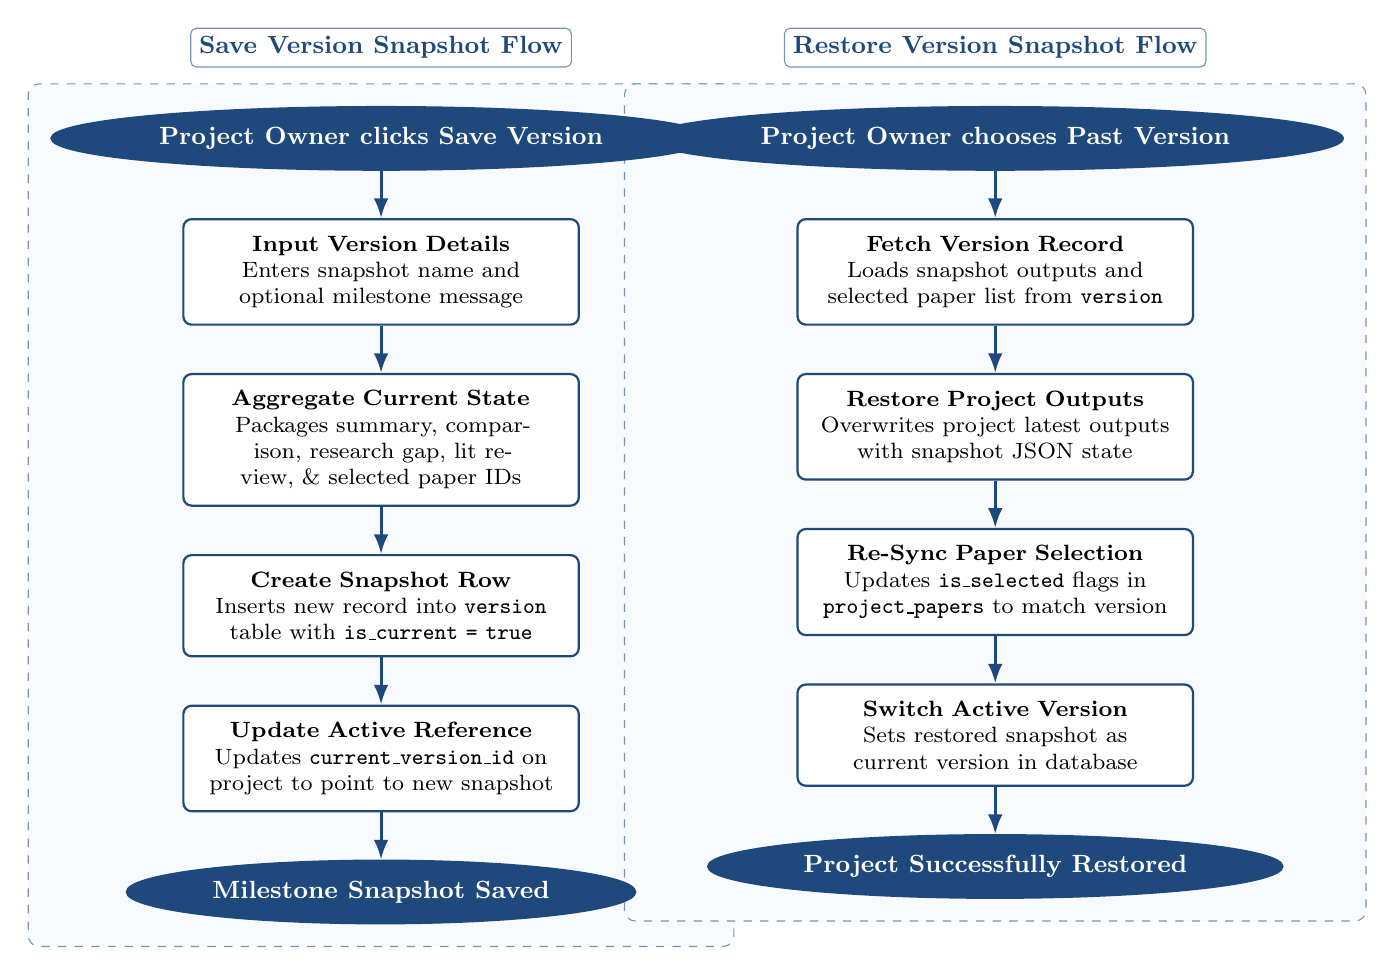
\begin{tikzpicture}[
    every node/.style={font=\small},
    phasebox/.style={
        rectangle, 
        draw=headerblue!60, 
        dashed, 
        fill=lightblue!10, 
        rounded corners=4pt, 
        inner sep=8pt
    },
    phasetitle/.style={
        font=\bfseries\small\color{headerblue}, 
        fill=white, 
        draw=headerblue!60, 
        rounded corners=2pt, 
        inner sep=3pt
    },
    startstop/.style={
        ellipse, 
        draw=headerblue, 
        thick, 
        fill=headerblue, 
        text=white, 
        font=\bfseries\small, 
        inner sep=4pt, 
        text centered
    },
    process/.style={
        rectangle, 
        draw=headerblue, 
        thick, 
        fill=white, 
        rounded corners=3pt, 
        text width=4.6cm, 
        text centered, 
        inner sep=6pt, 
        font=\footnotesize
    },
    arrow/.style={
        thick, 
        line width=1.1pt, 
        -{Latex[length=2.5mm]}, 
        draw=headerblue
    }
]

% ==================== LEFT: SAVE SNAPSHOT FLOW ====================
\node (s_start) [startstop] at (0, 0) {Project Owner clicks Save Version};
\node (s_input) [process, below=0.6cm of s_start] {\textbf{Input Version Details} \\ Enters snapshot name and optional milestone message};
\node (s_gather) [process, below=0.6cm of s_input] {\textbf{Aggregate Current State} \\ Packages summary, comparison, research gap, lit review, \& selected paper IDs};
\node (s_insert) [process, below=0.6cm of s_gather] {\textbf{Create Snapshot Row} \\ Inserts new record into \texttt{version} table with \texttt{is\_current = true}};
\node (s_link) [process, below=0.6cm of s_insert] {\textbf{Update Active Reference} \\ Updates \texttt{current\_version\_id} on project to point to new snapshot};
\node (s_end) [startstop, below=0.6cm of s_link] {Milestone Snapshot Saved};

\draw [arrow] (s_start) -- (s_input);
\draw [arrow] (s_input) -- (s_gather);
\draw [arrow] (s_gather) -- (s_insert);
\draw [arrow] (s_insert) -- (s_link);
\draw [arrow] (s_link) -- (s_end);


% ==================== RIGHT: RESTORE VERSION FLOW ====================
\node (r_start) [startstop] at (7.8, 0) {Project Owner chooses Past Version};
\node (r_fetch) [process, below=0.6cm of r_start] {\textbf{Fetch Version Record} \\ Loads snapshot outputs and selected paper list from \texttt{version}};
\node (r_restore) [process, below=0.6cm of r_fetch] {\textbf{Restore Project Outputs} \\ Overwrites project latest outputs with snapshot JSON state};
\node (r_sync) [process, below=0.6cm of r_restore] {\textbf{Re-Sync Paper Selection} \\ Updates \texttt{is\_selected} flags in \texttt{project\_papers} to match version};
\node (r_active) [process, below=0.6cm of r_sync] {\textbf{Switch Active Version} \\ Sets restored snapshot as current version in database};
\node (r_end) [startstop, below=0.6cm of r_active] {Project Successfully Restored};

\draw [arrow] (r_start) -- (r_fetch);
\draw [arrow] (r_fetch) -- (r_restore);
\draw [arrow] (r_restore) -- (r_sync);
\draw [arrow] (r_sync) -- (r_active);
\draw [arrow] (r_active) -- (r_end);

% Background grouping boxes
\begin{scope}[on background layer]
    \node (box_s) [phasebox, fit=(s_start) (s_end)] {};
    \node (title_s) [phasetitle, above=0.2cm of box_s.north] {\textsc{Save Version Snapshot Flow}};

    \node (box_r) [phasebox, fit=(r_start) (r_end)] {};
    \node (title_r) [phasetitle, above=0.2cm of box_r.north] {\textsc{Restore Version Snapshot Flow}};
\end{scope}

\end{tikzpicture}%
}
\caption{Activity Diagram for Project Version Snapshot Creation and Rollback Restoration.}
\label{fig:activity_version}
\end{figure}

% ==============================================================================
% 5. TECHNOLOGIES AND INTEGRATIONS
% ==============================================================================
\section{Technologies and Integrations}

\subsection{Frontend Framework: Flutter (Dart)}
\textbf{Why chosen:} Flutter was selected because it allows building cross-platform applications from a single codebase. Flutter's reactive UI framework and extensive widget library made it straightforward to build multi-pane responsive interfaces (such as side-by-side paper comparison views and split-screen Markdown editors) while maintaining consistent UI performance across platforms. Compared to React or traditional HTML/CSS stacks, Flutter gave us strict compile-time typing and a single language for all client-side logic.

\subsection{Backend Framework: FastAPI (Python 3.11)}
\textbf{Why chosen:} Python is the standard language for AI and natural language processing libraries. FastAPI was chosen over Flask and Django because it natively supports asynchronous I/O, provides automatic OpenAPI documentation, and enforces strict request/response data validation via Pydantic models. FastAPI's lightweight architecture allows fast cold-starts and clean endpoint organization for our multi-agent pipeline.

\subsection{Multi-Agent Pipeline: LangGraph and Google GenAI SDK}
\textbf{Why chosen:} Rather than building rigid, hard-coded prompt sequences, we used \textbf{LangGraph} to represent research agents as modular graph nodes operating over a shared state object (\texttt{LiteratureReviewState}). This allows the system to support flexible entry and exit points depending on what the user wants to do. \textbf{Google Gemini 2.0 Flash} was selected as the underlying LLM via the official \texttt{google-genai} SDK because of its fast inference speeds, large context window (handling numerous full academic abstracts simultaneously), and cost-effective pricing for iterative research tasks.

\subsection{Academic Paper Database: Semantic Scholar Graph API}
\textbf{Why chosen:} Many public academic APIs (such as arXiv) only cover specific disciplines like physics and computer science, and often lack citation metrics. Semantic Scholar covers all major academic fields, provides rich metadata (including citation counts, DOIs, open-access PDF links, and publication years), and offers a well-structured REST API with keyword query support.

\subsection{Database and Authentication: Supabase (PostgreSQL)}
\textbf{Why chosen:} Supabase provides managed PostgreSQL with built-in user authentication (GoTrue) and instant RESTful API access via PostgREST. Using Supabase eliminated the need to maintain an independent authentication server or database migration infrastructure, allowing our backend to interact securely with relational tables via service-role keys while leveraging PostgreSQL features like JSONB and foreign-key constraints.

\clearpage
% ==============================================================================
% 6. CUSTOM LOGIC AND ALGORITHMIC IMPLEMENTATIONS
% ==============================================================================
\section{Custom Logic and Algorithmic Implementations}

ScholarFlow incorporates several custom algorithms and logic routines designed specifically for academic research tasks.

\subsection{Paper Deduplication and Citation-Based Ranking}
When searching across multiple queries generated by the Query Planning Agent, different queries frequently return overlapping papers. Furthermore, some papers may share identical titles with slightly different punctuation or missing DOIs. 

To solve this, we implemented a custom two-tier deduplication algorithm in \texttt{Search\_Agent.py}. The algorithm normalizes paper titles by stripping non-alphanumeric characters and converting text to lowercase. It then performs set-based deduplication against both lowercase DOIs and normalized title keys. Finally, it sorts the unique papers in descending order by citation count so the most impactful papers appear first.

\begin{lstlisting}[language=Python, caption={Paper Deduplication and Citation Ranking in Search\_Agent.py}]
def _normalize_title(title: str) -> str:
    return "".join(ch.lower() for ch in title if ch.isalnum())

def deduplicate_papers(papers: List[Dict]) -> List[Dict]:
    seen_doi, seen_title, unique = set(), set(), []
    for p in papers:
        if not p.get("title"):
            continue
        doi = (p.get("doi") or "").lower()
        title_key = _normalize_title(p["title"])
        if doi and doi in seen_doi:
            continue
        if title_key in seen_title:
            continue
        seen_doi.add(doi)
        seen_title.add(title_key)
        unique.append(p)
    # Sort remaining unique papers by highest citation count first
    return sorted(unique, key=lambda p: p.get("citations", 0), reverse=True)
\end{lstlisting}

\subsection{Adaptive Request Throttling and Exponential Backoff}
The Semantic Scholar API enforces strict rate limits. Making multiple rapid queries frequently causes HTTP 429 (Too Many Requests) errors. To prevent runtime crashes and ensure reliable search operations, we implemented adaptive request throttling combined with exponential backoff retry logic.

\begin{lstlisting}[language=Python, caption={Throttling and Retry Mechanism in Search\_Agent.py}]
SEMANTIC_REQUEST_INTERVAL_SECONDS = 1.1
_last_semantic_request_ts = 0.0

def _throttle_semantic_scholar_requests() -> None:
    global _last_semantic_request_ts
    now = time.monotonic()
    elapsed = now - _last_semantic_request_ts
    if elapsed < SEMANTIC_REQUEST_INTERVAL_SECONDS:
        time.sleep(SEMANTIC_REQUEST_INTERVAL_SECONDS - elapsed)
    _last_semantic_request_ts = time.monotonic()

def _retry(fn, *args, **kwargs) -> Optional[requests.Response]:
    last_err = None
    for attempt in range(1, MAX_RETRIES + 1):
        try:
            resp = fn(*args, **kwargs)
            resp.raise_for_status()
            return resp
        except Exception as e:
            last_err = e
            status_code = getattr(getattr(e, "response", None), "status_code", None)
            if status_code == 429:
                time.sleep(3 * attempt) # Longer backoff for rate limits
            else:
                time.sleep(1.5 * attempt)
    print(f"[SearchAgent] Request failed after {MAX_RETRIES} retries: {last_err}")
    return None
\end{lstlisting}

\subsection{Intent Routing and Dynamic Graph Segment Execution}
Instead of forcing users through all six agents every time they run a command, ScholarFlow uses a Router Agent (\texttt{Router\_Agent.py}) to classify user requests and determine the exact start and end nodes required in the LangGraph workflow. If the LLM routing call fails, a rule-based token matching fallback determines the proper execution path.

\begin{lstlisting}[language=Python, caption={Workflow State and Dynamic Routing in workflow.py}]
def build_langgraph_workflow(start_node: str, end_node: str):
    graph = StateGraph(LiteratureReviewState)
    graph.add_node("query_planning", query_planning_agent)
    graph.add_node("search", search_agent)
    graph.add_node("summary", summary_agent)
    graph.add_node("comparison", comparison_agent)
    graph.add_node("research_gap", research_gap_agent)
    graph.add_node("literature_review", literature_review_agent)

    graph.add_edge(START, start_node)
    ordered_nodes = list(GRAPH_NODE_ORDER)
    start_index = ordered_nodes.index(start_node)
    end_index = ordered_nodes.index(end_node)

    if start_index <= end_index:
        for idx in range(start_index, end_index):
            graph.add_edge(ordered_nodes[idx], ordered_nodes[idx + 1])
        graph.add_edge(ordered_nodes[end_index], END)
    else:
        graph.add_edge(start_node, END)
    return graph.compile()
\end{lstlisting}

\subsection{Role-Gated Section Ownership and Edit-Request Approval Logic}
To prevent collaborative write collisions, our backend enforces a two-tier editing model in \texttt{main.py}. The project owner alone assigns section ownership. When a non-owner attempts to edit a section, the backend directs their draft to an edit request queue. The section owner can then review the proposed content and execute an approval endpoint that updates the live approved content.

\begin{lstlisting}[language=Python, caption={Edit Request Approval Logic in main.py}]
@app.post("/projects/{project_id}/sections/{section_key}/edit-requests/{request_id}/approve")
def approve_section_edit_request(
    project_id: str, section_key: str, request_id: str, payload: ResolveSectionEditRequest
) -> dict:
    _ensure_supabase()
    key = _require_valid_section_key(section_key)
    # Ensure caller is the assigned section owner
    actor = _require_section_owner(project_id, key, payload.actor_user_id)
    edit_request = supabase_service.get_section_edit_request(request_id)
    
    if not edit_request or edit_request.get("status") != "pending":
        raise HTTPException(status_code=400, detail="Invalid or resolved request.")
        
    resolved = supabase_service.resolve_section_edit_request(request_id, "approved", actor)
    # Promote proposed content to the live section
    section = supabase_service.update_section_content(
        project_id, key, edit_request.get("proposed_content", ""), actor
    )
    return {"edit_request": resolved, "section": section}
\end{lstlisting}

% ==============================================================================
% 7. CHALLENGES AND SOLUTIONS
% ==============================================================================
\section{Challenges and Solutions}

During the development of ScholarFlow, our team encountered several technical and design challenges:

\subsection{Handling Academic API Rate Limits (HTTP 429)}
\textbf{Challenge:} The Semantic Scholar API strictly enforces rate limits on free-tier requests. When our Query Planning Agent generated 4 to 6 query variations, executing them in parallel triggered frequent HTTP 429 exceptions, resulting in failed searches. \\
\textbf{Solution:} We introduced a client-side timestamp throttle (\texttt{time.monotonic()}) ensuring a mandatory delay of at least 1.1 seconds between requests, plus a 2-second sleep between query batches. We also added an exponential retry wrapper that catches HTTP 429 status codes and backs off before retrying.

\subsection{LLM JSON Schema Inconsistencies}
\textbf{Challenge:} Large language models often wrap JSON responses in Markdown code blocks (e.g., \verb|```json ... ```|) or include conversational filler before or after the JSON payload. This caused \texttt{json.loads()} to fail frequently in early agent prototypes. \\
\textbf{Solution:} We wrote a robust helper function (\texttt{extract\_json} in \texttt{agent\_utils.py}) that uses regex to strip code fences and searches for the first opening brace \verb|{| and last closing brace \verb|}|. This allows the system to cleanly parse valid JSON even if the model outputs conversational text around it.

\subsection{Collaborative Document Write Collisions}
\textbf{Challenge:} In team research projects, multiple students often try to edit the same section simultaneously. A simple ``last write wins'' approach caused teammates to unintentionally overwrite each other's work. \\
\textbf{Solution:} We designed a role-gated workflow model. Each section has a designated owner who has direct write access. Other collaborators are restricted to saving local working copies in a split-view editor and submitting formal edit requests. This guarantees that approved section content is never modified without explicit review.

\subsection{Database ID Format Consistency (UUID vs. Integer)}
\textbf{Challenge:} Early iterations of our database schema mixed auto-incrementing integer IDs with Supabase UUID strings, leading to type errors in foreign-key lookups when passing parameters from the Flutter client to FastAPI. \\
\textbf{Solution:} We standardized all primary and foreign keys across all database tables to UUID strings (\texttt{gen\_random\_uuid()}), updated all Pydantic models to accept string IDs, and removed all numeric ID casts across the backend service layer.

% ==============================================================================
% 8. FUTURE IMPROVEMENTS
% ==============================================================================
\section{Future Improvements}

While ScholarFlow is currently fully functional, there are several areas planned for future development:

\begin{itemize}
    \item \textbf{Full-Text PDF Extraction and Parsing:} The current pipeline relies on paper abstracts. Integrating a PDF ingestion service (such as Grobid or PyMuPDF) would allow agents to analyze specific experimental tables, datasets, and mathematical formulations from full paper bodies.
    \item \textbf{Real-Time Collaborative Cursor Editing:} Currently, collaboration works through working drafts and edit requests. Implementing WebSockets with operational transformation (OT) or Conflict-Free Replicated Data Types (CRDTs) would enable real-time Google Docs-style simultaneous editing for section co-authors.
    \item \textbf{Direct LaTeX and BibTeX Export:} Adding an automated export tool that compiles project sections, references, and comparison tables into downloadable `.tex` and `.bib` archives ready for submission to conferences (e.g., IEEE, ACM) or Overleaf.
    \item \textbf{Citation Network Graph Visualization:} Incorporating an interactive node-link graph on the frontend showing citation pathways and co-authorship clusters between retrieved papers to help researchers spot foundational papers visually.
\end{itemize}

\end{document}
